\section{突现推理行为}

\subsection{与 LLM 行为的类比}

论文发现，视频扩散模型中出现了一些与 LLM 早期推理研究相似的突现行为。它们不是通过显式文本推理链表现出来，而是体现在 latent 随 diffusion steps 演化的动态中。主要包括工作记忆、自我修正与增强，以及先感知后行动。

\subsection{工作记忆}

工作记忆指模型在推理过程中保持关键信息的能力。对视频任务来说，这尤其重要，因为目标可能被遮挡、消失或移动，但模型仍需要保持对象身份和初始位置。

Figure~\ref{fig:figure4} 中的 object reappearance 示例显示，模型能在整个扩散过程中保留物体的初始位置，使圆能够回到原点。Teddy bear relocation 示例中，大熊一度遮挡小熊，但模型在早期步骤已经保存了小熊信息，因此后续生成仍能保持一致。

\begin{figure}[H]
    \centering
    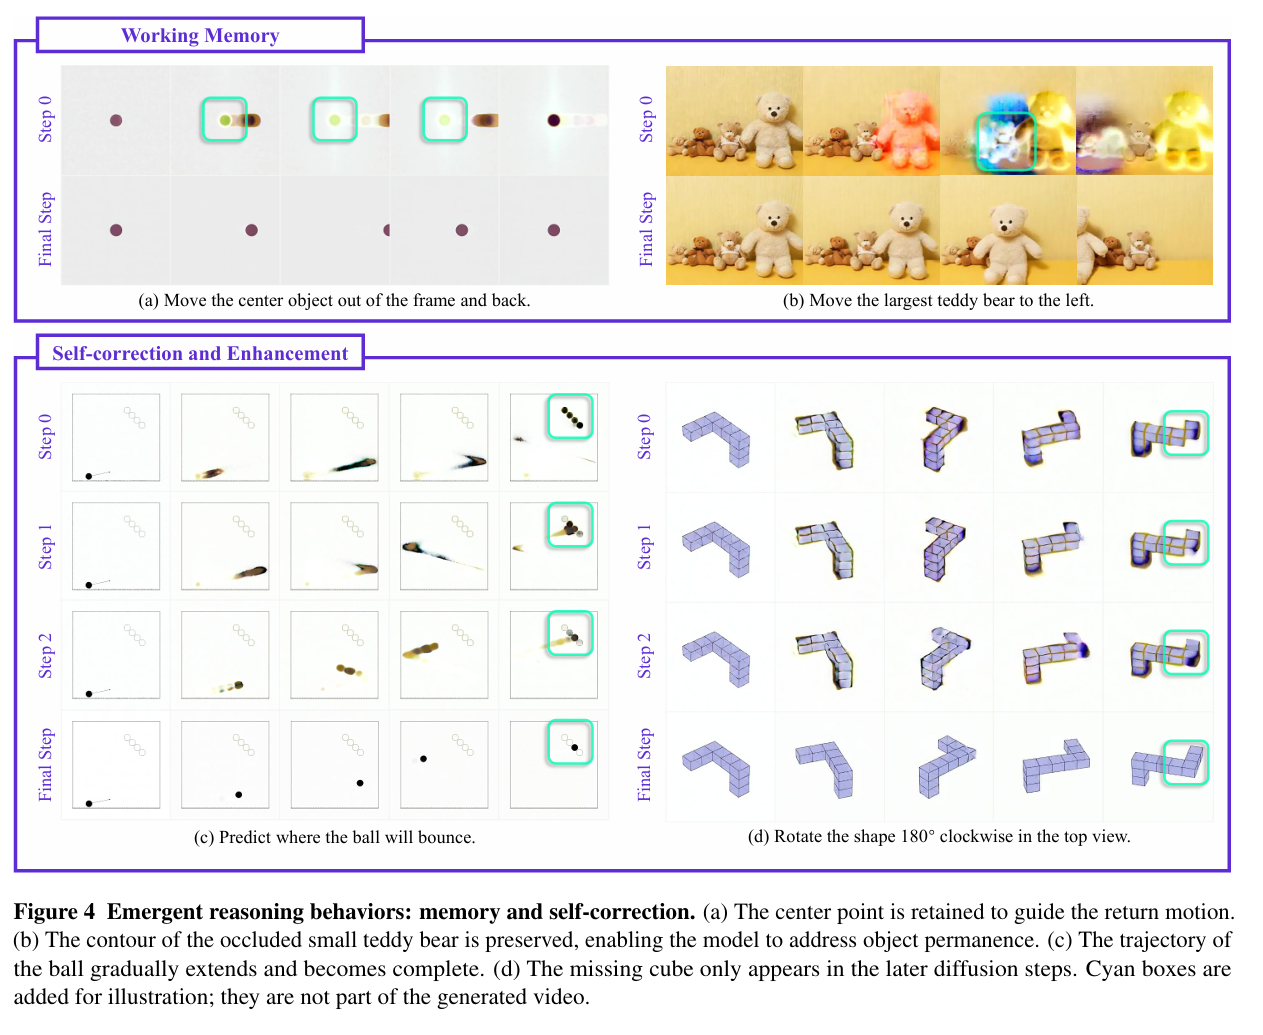
\includegraphics[width=0.96\textwidth]{figures/figure4.png}
    \caption{视频扩散模型中的突现推理行为：工作记忆、自我修正与增强。}
    \label{fig:figure4}
\end{figure}

这说明扩散过程中的 latent 不是只保存当前可见像素，而是能形成某些稳定锚点，用来跨步骤、跨帧维持任务相关状态。

\subsection{自我修正与增强}

自我修正指模型早期可能产生错误候选，但后续 diffusion steps 能够纠正错误并切换到更合理的策略。与 CoF 逐帧推进不同，这种修正往往在同一个 step 内对所有帧全局发生。

例如 hit target after bounce 任务中，初始轨迹可能模糊且包含多个候选反弹点，后续步骤逐渐筛掉错误轨迹，最终收敛到正确命中点。3D shape rotation 任务中，模型早期可能在数量或排列上出错，但随后逐步修正，形成正确结构。

这类行为类似 LLM 中的 backtracking 或 slow thinking，但在视频扩散模型中没有显式文本回溯，而是通过 latent 轨迹的重写和剪枝体现。

\subsection{先感知后行动}

先感知后行动指模型早期优先解决“是什么”和“在哪里”，后期再决定“怎么移动”或“如何操作”。Figure~\ref{fig:figure5} 展示了这种从静态感知到动态推理的转变。

\begin{figure}[H]
    \centering
    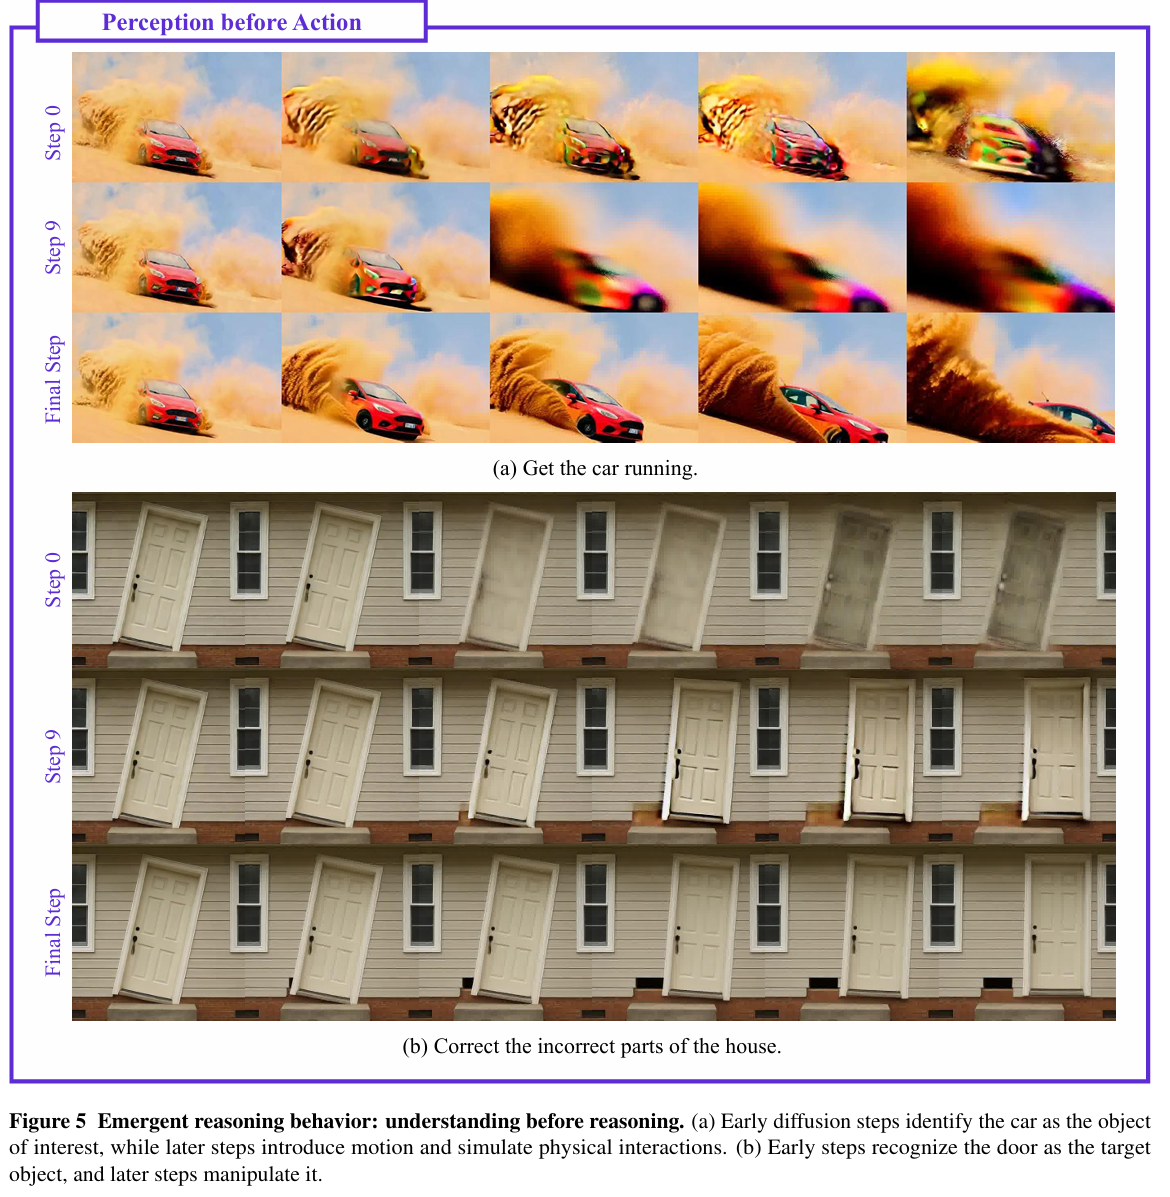
\includegraphics[width=0.96\textwidth]{figures/figure5.png}
    \caption{先感知后行动：早期步骤定位目标，后续步骤再进行运动规划和关系推理。}
    \label{fig:figure5}
\end{figure}

直观地说，模型先建立场景中有哪些前景目标、目标在哪里、背景结构如何；随后才生成运动轨迹、交互关系或操作行为。这个顺序很合理，因为复杂行动依赖稳定的目标定位和场景理解。

\subsection{这三类行为与 CoS 的关系}

工作记忆、自我修正、先感知后行动都说明：视频推理不是一次性完成，也不是简单逐帧传递。它更像一个多轮全局 refinement 过程：

\begin{itemize}
    \item 工作记忆保证关键对象和关系能跨步骤保留。
    \item 自我修正说明早期错误并非不可逆，后续步骤仍可修改全局假设。
    \item 先感知后行动说明不同阶段承担不同功能，推理具有阶段性。
\end{itemize}

这些现象共同支持 CoS：扩散步骤不仅让画面变清晰，也让推理状态逐步演化。
